\documentclass[tikz,border=8pt]{standalone}
% Shared look for every TikZ diagram. Load with \input{../../tools/tikz-style.tex}
\usepackage[T1]{fontenc}
\usepackage{lmodern}
\renewcommand{\sfdefault}{lmr}  % diagrams use the same serif as the text
\usetikzlibrary{arrows.meta, positioning, shapes.geometric, calc, fit, backgrounds}
\definecolor{cblue}{HTML}{4C78A8}
\definecolor{corange}{HTML}{F58518}
\definecolor{cgreen}{HTML}{54A24B}
\definecolor{cred}{HTML}{E45756}
\definecolor{cpurple}{HTML}{B279A2}
\definecolor{cgrey}{HTML}{6B6B6B}
\tikzset{
  every picture/.style={font=\sffamily, line width=1.2pt},
  box/.style={draw=#1, fill=#1!12, rounded corners=4pt, align=center, inner sep=7pt, minimum height=1.1cm},
  box/.default=cgrey,
  arrow/.style={-{Stealth[length=3mm]}, draw=cgrey, line width=1.4pt},
  title/.style={font=\sffamily\bfseries\Large},
  note/.style={font=\sffamily\small, text=cgrey, align=center},
}
\AtBeginDocument{\hyphenpenalty=10000 \exhyphenpenalty=10000}

% Placing a pose from one reading (r, phi) of the pink pole m = (4.4, 3.8). Pick an angle gamma around the pole;
% the robot sits at m + r (cos gamma, sin gamma). From the robot the pole lies in the direction gamma + 180 deg.
% The bearing phi is that direction minus the heading, so theta = gamma + 180 deg - phi.
% Drawn with r = 3.0, phi = 36.87 deg and gamma = 216.87 deg, which gives the pose (2, 2, 0).
\begin{document}
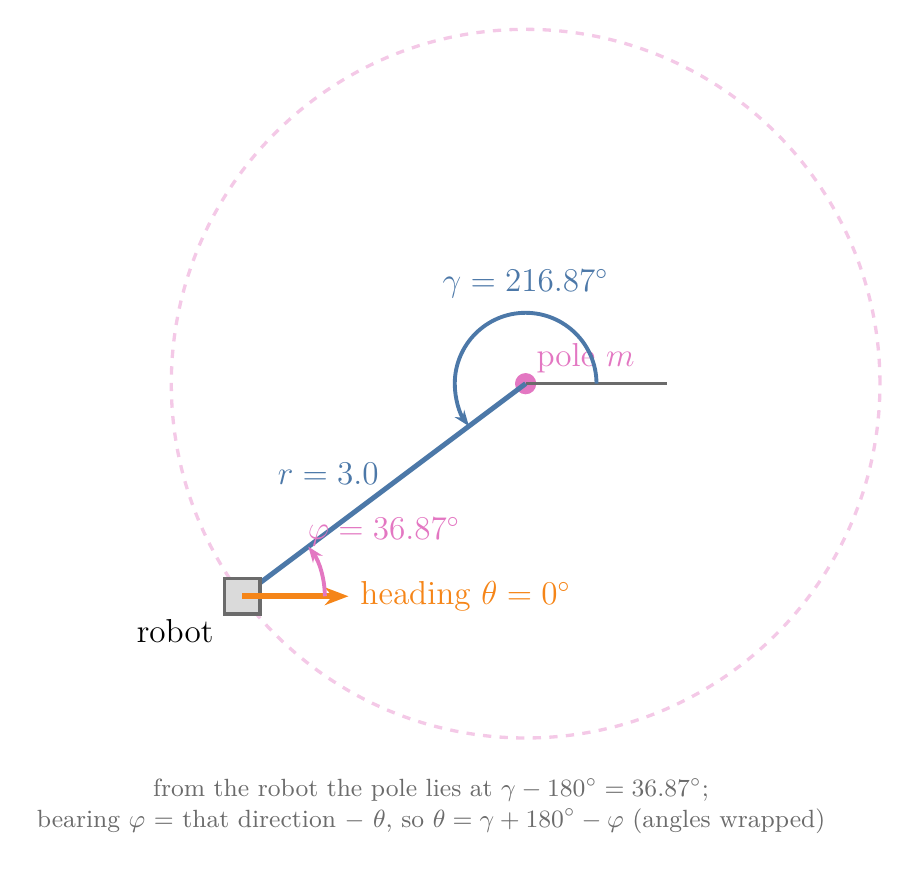
\begin{tikzpicture}[scale=1.5, every node/.append style={font=\large}]
  \definecolor{cpink}{HTML}{E377C2}
  \draw[cpink!40, line width=1.2pt, dashed] (4.4,3.8) circle (3.0);
  \fill[cpink] (4.4,3.8) circle (0.09); \node[cpink, above right] at (4.4,3.8) {pole $m$};
  \draw[cgrey, line width=1pt] (4.4,3.8) -- (5.6,3.8);
  \draw[cblue, line width=1.4pt, -{Stealth[length=2mm]}] (5.0,3.8) arc (0:216.87:0.6);
  \node[cblue] at (4.4,4.65) {$\gamma = 216.87^\circ$};
  \draw[cblue, line width=1.8pt] (4.4,3.8) -- (2,2) node[midway, above left, fill=white, inner sep=1pt] {$r = 3.0$};
  \draw[cgrey, fill=cgrey!25] (1.85,1.85) rectangle (2.15,2.15);
  \draw[-{Stealth[length=3mm]}, corange, line width=2pt] (2,2) -- (2.9,2) node[right] {heading $\theta = 0^\circ$};
  \draw[cpink, line width=1.4pt, -{Stealth[length=2mm]}] (2.7,2) arc (0:36.87:0.7);
  \node[cpink] at (3.2,2.55) {$\varphi = 36.87^\circ$};
  \node[below left] at (1.85,1.9) {robot};
  \node[note, anchor=north, align=center] at (3.6,0.55) {from the robot the pole lies at $\gamma - 180^\circ = 36.87^\circ$;\\ bearing $\varphi$ = that direction $-$ $\theta$, so $\theta = \gamma + 180^\circ - \varphi$ (angles wrapped)};
\end{tikzpicture}
\end{document}
